\documentclass{standalone}

\usepackage[english]{babel}
\usepackage[utf8x]{inputenc}
\usepackage[T1]{fontenc}
\usepackage{tikz,pgf} %and any other packages or tikzlibraries your picture needs
\usepackage{amsfonts}
\usepackage{amsmath}
\usepackage{physics}
\usepackage{amssymb}
\usepackage{mathtools}
\usetikzlibrary{shapes,arrows,patterns}

\begin{document}

%%%%%%%%%%%%%%%%%%%%%%%%%%%%%%%%%%%%%%%%%%%%%%%%%%%%%%%%%%%%%%%%%%%%%%%%%%%%%%%%
%COPY HERE
%%%%%%%%%%%%%%%%%%%%%%%%%%%%%%%%%%%%%%%%%%%%%%%%%%%%%%%%%%%%%%%%%%%%%%%%%%%%%%%%



\tikzset{every picture/.style={line width=0.75pt}} %set default line width to 0.75pt

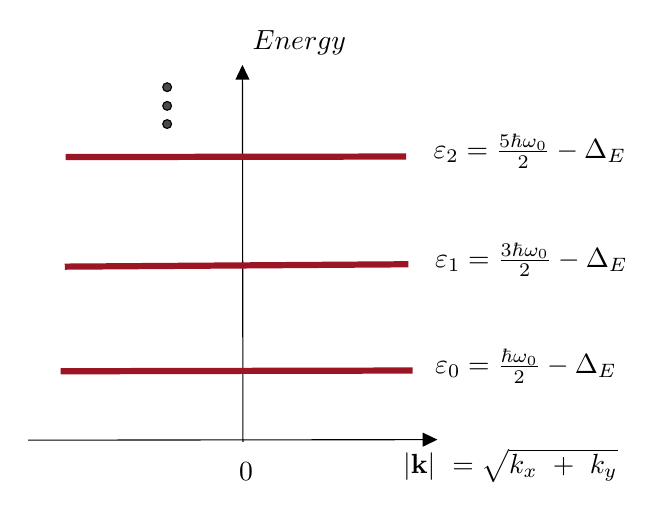
\begin{tikzpicture}[x=0.75pt,y=0.75pt,yscale=-1,xscale=1]
%uncomment if require: \path (0,338); %set diagram left start at 0, and has height of 338

%Straight Lines [id:da05241196214452626]
\draw    (238.65,205.45) -- (238.4,26.8) ;
\draw [shift={(238.4,23.8)}, rotate = 449.92] [fill={rgb, 255:red, 0; green, 0; blue, 0 }  ][line width=0.08]  [draw opacity=0] (7.14,-3.43) -- (0,0) -- (7.14,3.43) -- cycle    ;
%Straight Lines [id:da6020218277675191]
\draw    (135.2,204.6) -- (329.35,204.35) ;
\draw [shift={(332.35,204.35)}, rotate = 539.9300000000001] [fill={rgb, 255:red, 0; green, 0; blue, 0 }  ][line width=0.08]  [draw opacity=0] (7.14,-3.43) -- (0,0) -- (7.14,3.43) -- cycle    ;
%Straight Lines [id:da9431959114242063]
\draw [color={rgb, 255:red, 156; green, 21; blue, 37 }  ,draw opacity=1 ][line width=2.25]    (150.8,171.4) -- (320.35,171.05) ;
%Straight Lines [id:da37284196508889367]
\draw [color={rgb, 255:red, 156; green, 21; blue, 37 }  ,draw opacity=1 ][line width=2.25]    (152.8,121) -- (318.35,119.85) ;
%Straight Lines [id:da4935257751480193]
\draw [color={rgb, 255:red, 156; green, 21; blue, 37 }  ,draw opacity=1 ][line width=2.25]    (153.2,68.2) -- (317.25,67.95) ;
%Shape: Circle [id:dp8412837697747655]
\draw  [fill={rgb, 255:red, 74; green, 74; blue, 74 }  ,fill opacity=1 ] (200,52.29) .. controls (200,51.12) and (200.95,50.17) .. (202.13,50.17) .. controls (203.3,50.17) and (204.25,51.12) .. (204.25,52.29) .. controls (204.25,53.47) and (203.3,54.42) .. (202.13,54.42) .. controls (200.95,54.42) and (200,53.47) .. (200,52.29) -- cycle ;
%Shape: Circle [id:dp4130226792773326]
\draw  [fill={rgb, 255:red, 74; green, 74; blue, 74 }  ,fill opacity=1 ] (200,43.54) .. controls (200,42.37) and (200.95,41.42) .. (202.13,41.42) .. controls (203.3,41.42) and (204.25,42.37) .. (204.25,43.54) .. controls (204.25,44.72) and (203.3,45.67) .. (202.13,45.67) .. controls (200.95,45.67) and (200,44.72) .. (200,43.54) -- cycle ;
%Shape: Circle [id:dp6072986416723454]
\draw  [fill={rgb, 255:red, 74; green, 74; blue, 74 }  ,fill opacity=1 ] (200,34.54) .. controls (200,33.37) and (200.95,32.42) .. (202.13,32.42) .. controls (203.3,32.42) and (204.25,33.37) .. (204.25,34.54) .. controls (204.25,35.72) and (203.3,36.67) .. (202.13,36.67) .. controls (200.95,36.67) and (200,35.72) .. (200,34.54) -- cycle ;


% Text Node
\draw (235.5,214.4) node [anchor=north west][inner sep=0.75pt]    {$0$};
% Text Node
\draw (314.6,207.3) node [anchor=north west][inner sep=0.75pt]    {$|\mathbf{k} |\ =\sqrt{k_{x} \ +\ k_{y}}$};
% Text Node
\draw (242,6.13) node [anchor=north west][inner sep=0.75pt]    {$Energy$};
% Text Node
\draw (330,159.4) node [anchor=north west][inner sep=0.75pt]    {$\varepsilon _{0} =\frac{\hbar \omega _{0}}{2} -\Delta _{E}$};
% Text Node
\draw (330,108.2) node [anchor=north west][inner sep=0.75pt]    {$\varepsilon _{1} =\frac{3\hbar \omega _{0}}{2} -\Delta _{E}$};
% Text Node
\draw (329.2,55.8) node [anchor=north west][inner sep=0.75pt]    {$\varepsilon _{2} =\frac{5\hbar \omega _{0}}{2} -\Delta _{E}$};


\end{tikzpicture}


%%%%%%%%%%%%%%%%%%%%%%%%%%%%%%%%%%%%%%%%%%%%%%%%%%%%%%%%%%%%%%%%%%%%%%%%%%%%%%%%
%COPY HERE
%%%%%%%%%%%%%%%%%%%%%%%%%%%%%%%%%%%%%%%%%%%%%%%%%%%%%%%%%%%%%%%%%%%%%%%%%%%%%%%%

\end{document}
